\documentclass[a4paper,11pt ]{xc_webpage_project}
\usepackage[utf8]{inputenc}
\usepackage[spanish,english]{babel}
\usepackage{graphicx}
\usepackage[labelsep=period]{caption}
\usepackage{parallel}
\usepackage{wrapfig} %% Wrapping text around figures.
\usepackage{caption}
\usepackage{subcaption}

\renewcommand{\titProject}{FGT IWTE Plant. Quencher structural analysis}
\def\@anagramFont{\relax}
\renewcommand{\client}{AIT-STEIN / DEFISA}
\renewcommand{\dateProject}{2020}
\renewcommand{\location}{Jubail ind. city (KSA)}
\renewcommand{\widhtLeftCol}{0.475\textwidth} % normalmente no lo cambiaremos
\renewcommand{\widhtRightCol}{0.475\textwidth} % normalmente no lo cambiaremos


\begin{document}
\headerEnglish

\begin{Parallel}{\widhtLeftCol}{\widhtRightCol}
  \ParallelLText{The so-called Veolia Value Park (VVP) is a Integrated Waste To Energy (IWTE) Central Utilities and Valorization Plant that will precondition liquid and solid hazardous industrial waste (Class I and Class II), burning it and recovering energy in the form of steam for use within several industrial applications.
    
  }
  
  \ParallelRText{ \emph{El denominado Veolia Value Park (VVP) es una planta de tratamiento de residuos industriales peligrosos líquidos y sólidos (Clase I y Clase II), para recuperación de la energía generada en forma de vapor a través de la combustión de los  mismos.}
    
  }
\end{Parallel}

\begin{figure}[h]
  \begin{subfigure}[b]{\widhtLeftCol}
  \centering
  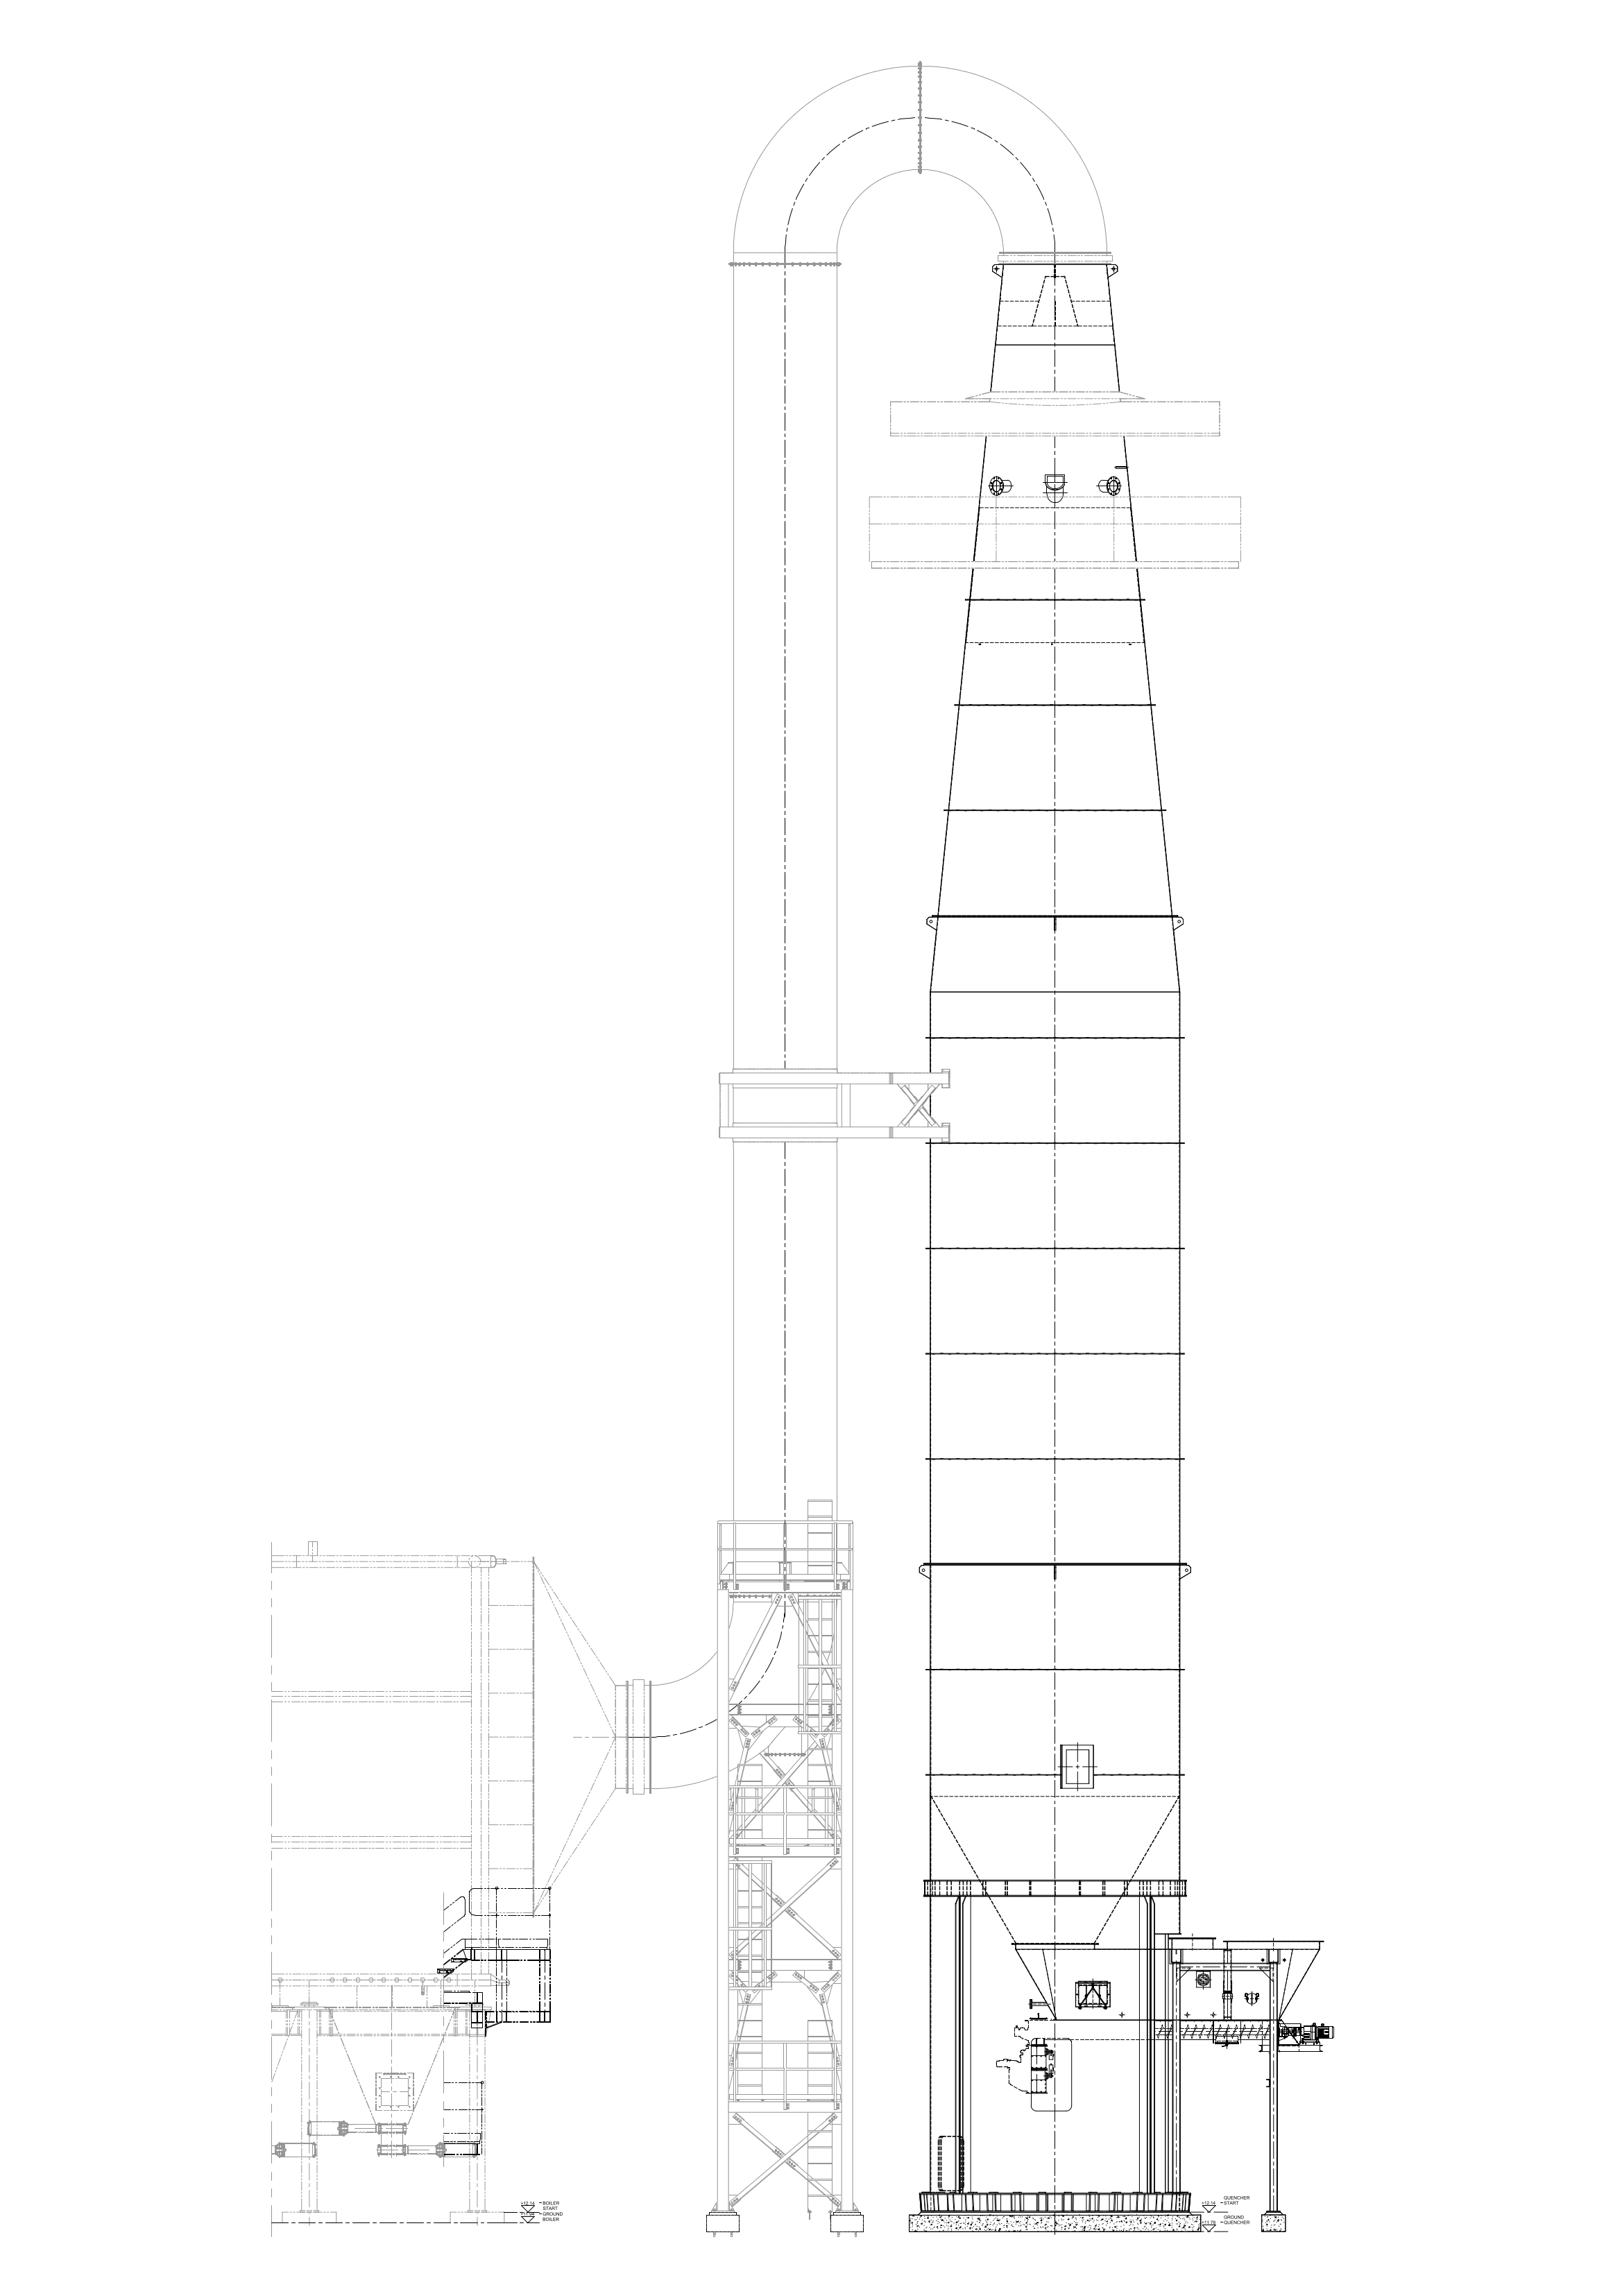
\includegraphics[width=\textwidth]{figures/quencher}
  \caption{Quencher and conduit boiler-quencher.}
  \end{subfigure}
\hfill
  \begin{subfigure}[b]{0.35\textwidth}
  \centering
  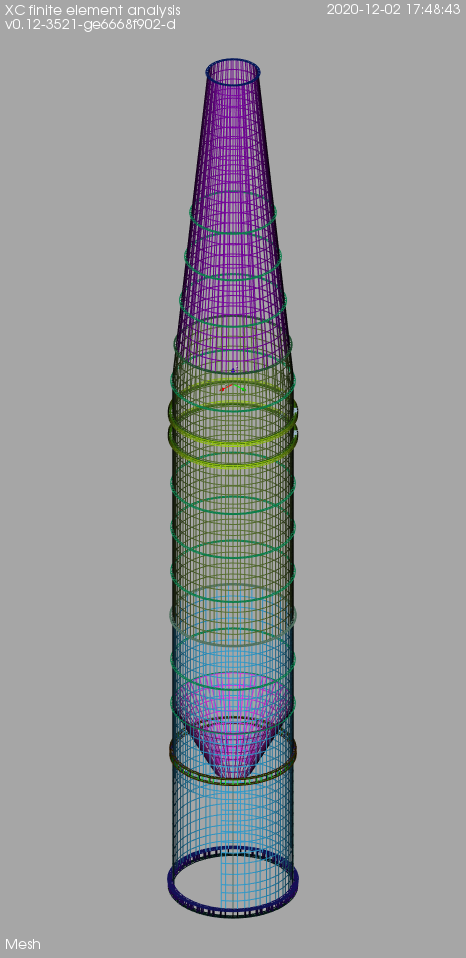
\includegraphics[width=\textwidth]{figures/model02}
  \caption{Finite element mesh}
  \end{subfigure}
  \end{figure}

\begin{Parallel}{\widhtLeftCol}{\widhtRightCol}
  \ParallelLText{    
    As part of the flue gas cleaning system, a quencher is designed. It  is the equipment that carries out the cooling of hot exhaust gas by water sprays before it enters the reactor. The structure is a cylindrical vessel of type column, 4.60 m in diameter and vertical height of 36.10 m. The shell thickness varies between 12 mm in the support skirt and 6 mm in the upper cone trunk.
  }
  
  \ParallelRText{     
     \emph{Integrado en el sistema de depuración de gases de combustión, se diseña un enfriador (quencher). Este es el equipo que enfría los gases procedentes de la caldera mediante aspersiones de agua, para su posterior incorporación al reactor. La estructura del enfriador es un tanque cilíndrico de tipo columna, de 4,60 m de diámetro y altura vertical de 36,10 m. El espesor de la pared varía entre 12 mm en el faldón de apoyo y 6 mm en el tronco del cono superior.}
  }
\end{Parallel}


\begin{Parallel}{\widhtLeftCol}{\widhtRightCol}
  \ParallelLText{
    At a height of approximately 21 m above the ground, the quencher structure is reinforced with two T-shaped ring stiffeners to accommodate the loads transmitted by the boiler conduit support.
    
    The quencher works at a temperature of 400$^o$C and is under external pressure (vacuum) equal to -7.84 kPa (-800 mmcda). The basic wind speed in the area is 155 $km/h$. The earthquake response acceleration has a value of $S_a = 0,091g$.
    
  }
  
  \ParallelRText  {\emph{A una altura aproximada de 21 m sobre el suelo, la estructura del enfriador se refuerza con dos rigidizadores anulares en forma de T para soportar las cargas transmitidas por el soporte del conducto proveniente de la caldera.}
    
     \emph{El enfriador trabaja a una temperatura de 400$^o$C y soporta una presión externa (vacío) igual a -7,84 kPa (-800 mmcda). La velocidad básica del viento en la zona es de 155 $km/h$. La aceleración sísmica de cálculo tiene un valor de $S_a = 0,091g$}
  }
\end{Parallel}


\begin{figure}[h]
  \begin{subfigure}[b]{\widhtLeftCol}
  \centering
  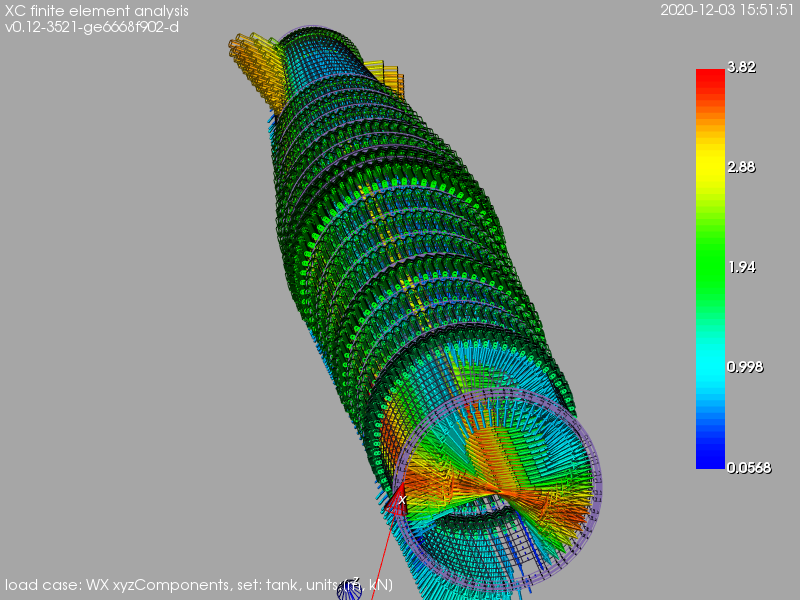
\includegraphics[width=\textwidth]{figures/quencher_WX_unif_det}
  \caption{Wind load pattern (bottom view)}
  \end{subfigure}
\hfill
  \begin{subfigure}[b]{\widhtRightCol}
  \centering
  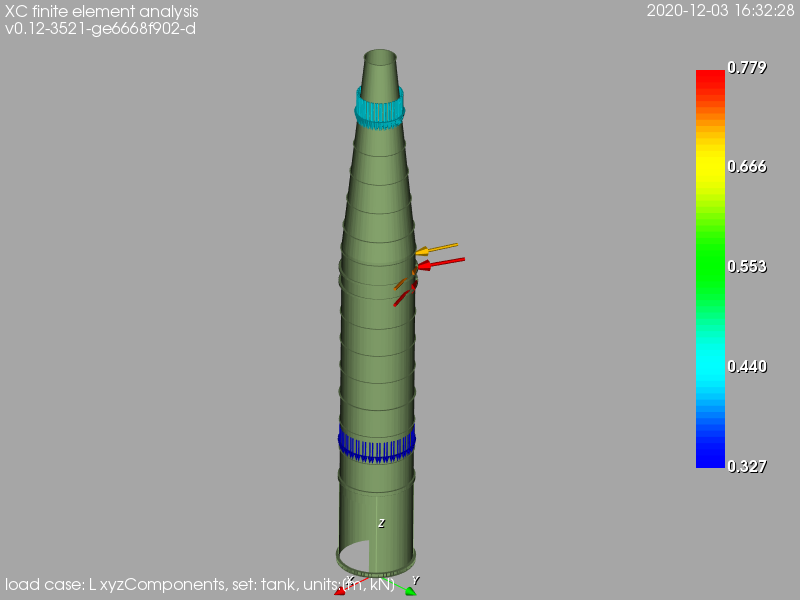
\includegraphics[width=\textwidth]{figures/quencher_L_point}
  \caption{ Live load pattern. }
  \end{subfigure}
  \end{figure}

\begin{Parallel}{\widhtLeftCol}{\widhtRightCol}
  \ParallelLText{To check the structure against plastic collapse, the analysis was conducted using The Design By Analysis (DBA) route proposed in the «ASME Pressure Vessel and Boiler Code». The reason is that the DBA-approach is more flexible than the methods based on Design By Formula, and simplifies the incorporation of constructional requirements (wind, earthquake, etc.) in a consistent manner. A limit-load analysis is applied to avoid the annoying problem of stress classification, since this method does not require categorization into primary and secondary stresses and it gives a unique result.

    To check the structure against collapse from buckling, an elastic-plastic analysis is performed on a FE model in which imperfections are explicitly considered. The geometry of the model with initial imperfections is created based on the maximum (admissible) out-of-roundness of the structure. A second-order analysis is performed using the nonlinear geometry and a linear-elastic ideal-plastic constitutive law.
  }
  
\ParallelRText  {\emph{Para verificar la estructura frente al colapso plástico, se realizó un anáisis siguiendo el procedimiento de «Design By Analysis» (DBA) propuesta en la norma «ASME Pressure Vessel and Boiler Code». La razón es que el enfoque DBA es más flexible que los métodos basados en \emph{Design By Formula} y simplifica la incorporación de requisitos de construcción (viento, terremoto, etc.) de manera consistente. Se aplica un análisis de carga límite para evitar la tedioso tarea de la clasificación de tensiones, ya que este método no requiere la categorización en tensiones primarias y secundarias y da un resultado único.}

     \emph{Para verificar la estructura contra el colapso por pandeo, se realiza un análisis elástico-plástico en un modelo FE en el que se consideran explícitamente las imperfecciones. La geometría del modelo con imperfecciones iniciales se crea en base al máximo ovalamiento admisible de la estructura. Se realiza un análisis de segundo orden utilizando la geometría no lineal y una ley constitutiva del material con comportamiento elastoplástico perfecto.}
  }
  
\end{Parallel}

\begin{figure}[h]
  \begin{subfigure}[b]{0.33\textwidth}
  \centering
  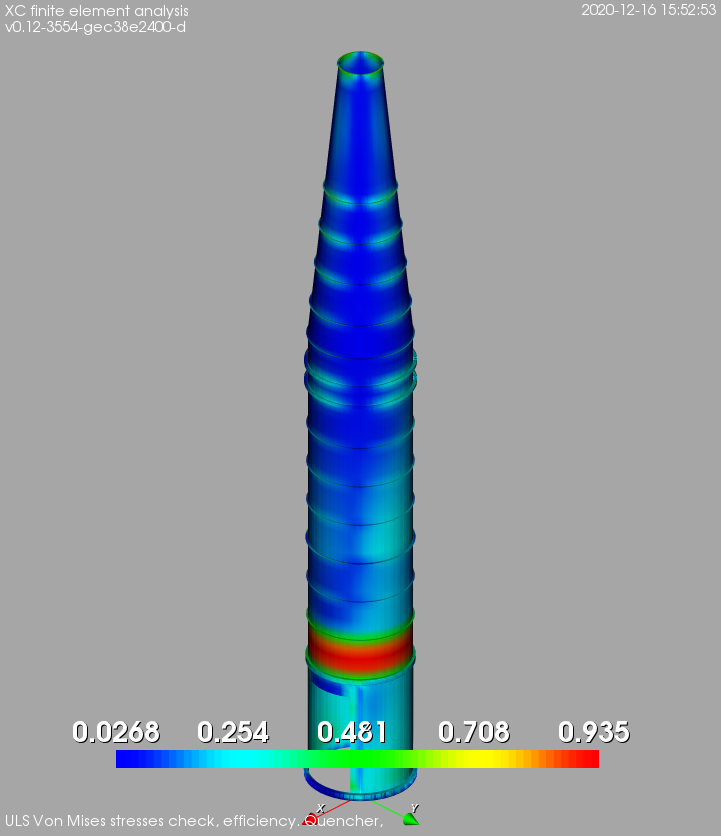
\includegraphics[width=\textwidth]{figures/LL01}
  \caption{Check against plastic collapse. Capacity factor}
  \end{subfigure}
\hfill
  \begin{subfigure}[b]{0.27\textwidth}
  \centering
  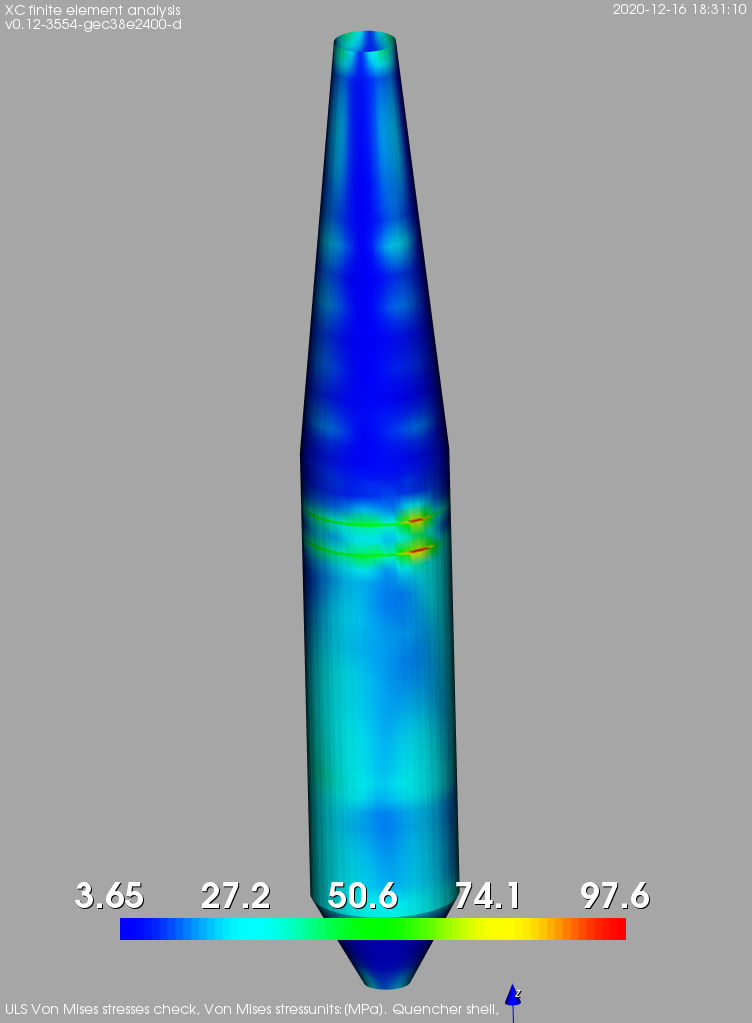
\includegraphics[width=\textwidth]{figures/vm_quencher_shell}
  \caption{Check against plastic collapse. Envelope of von-mises stresses in the quencher shell}
  \end{subfigure}
\hfill
  \begin{subfigure}[b]{0.30\textwidth}
  \centering
  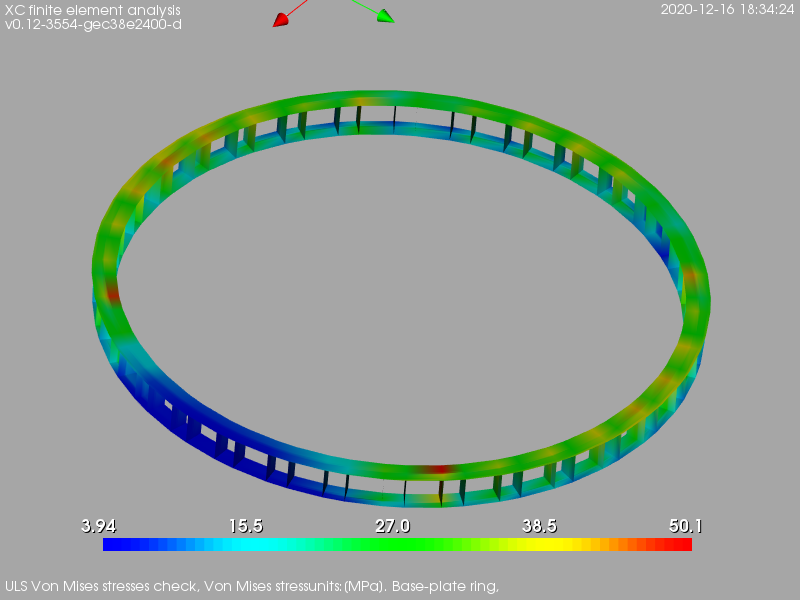
\includegraphics[width=\textwidth]{figures/vm_baseplate}
  \caption{Check against plastic collapse. Envelope of von-mises stresses in the base-plate ring}
  \end{subfigure}
\hfill
  \begin{subfigure}[b]{0.33\textwidth}
  \centering
  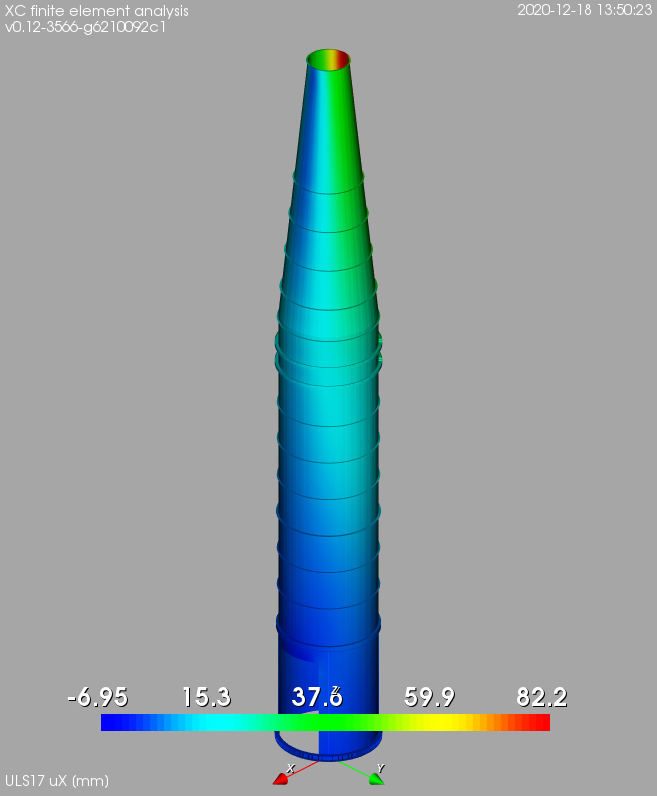
\includegraphics[width=\textwidth]{figures//uX_01}
  \caption{Check against collapse from buckling. Displacement in X direction. Front view}
  \end{subfigure}
\hfill
  \begin{subfigure}[b]{0.25\textwidth}
  \centering
  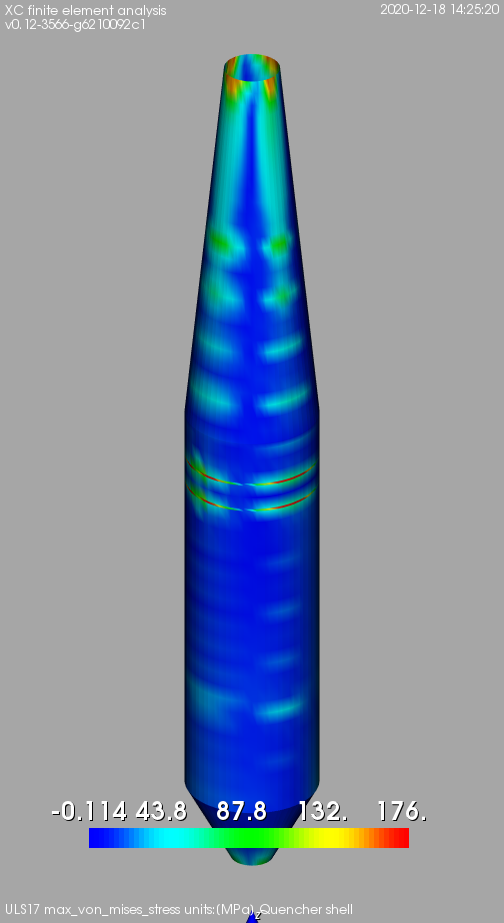
\includegraphics[width=\textwidth]{figures/vm_quencher_shell_buckling}
  \caption{Check against collapse from buckling.  Von-mises stresses in the quencher shell}
  \end{subfigure}
\hfill
  \begin{subfigure}[b]{0.30\textwidth}
  \centering
  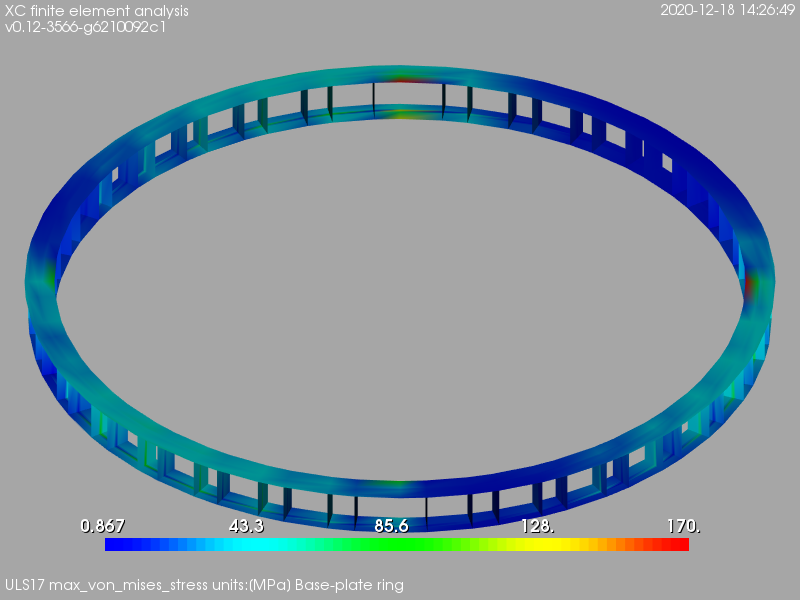
\includegraphics[width=\textwidth]{figures/vm_baseplate_buckling}
  \caption{Check against collapse from buckling. Von-mises stresses in the base-plate ring}
  \end{subfigure}
  \end{figure}

\end{document}

  
